\tikzstyle{vertex}=[circle, draw]
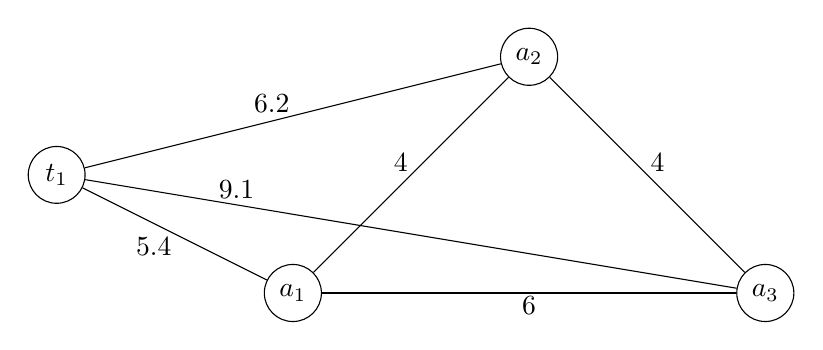
\begin{tikzpicture}[transform shape]
\node[vertex](a1) at (0, 0) {$ a_1 $};
\node[vertex](a2) at (3, 3) {$ a_2 $};
\node[vertex](a3) at (6, 0) {$ a_3 $};
\node[vertex](t1) at (-3,1.5) {$ t_1 $};

\begin{scope}[every path/.style={-}, every node/.style={inner sep=1pt}]
       \draw (a1) -- node [anchor=south east] {$4$} (a2);
       \draw (a2) -- node [anchor=south west] {$4$} (a3);
       \draw (a1) -- node [anchor=north] {$6$} (a3);
       \draw (t1) -- node [anchor=north east] {$5.4$} (a1);
       \draw (t1) -- node [anchor=south east] {$6.2$} (a2);
       \draw (t1) -- node [pos=0.2, anchor=south west] {$9.1$} (a3);
\end{scope} 
\end{tikzpicture}